\graphicspath{{chapters/chapter7/}}
\chapter{Appendix} \label{chapter7}
\section{Single-Task Learning}
\subsection{\texorpdfstring{\boldsymbol{$IncNet$}}{TEXT}}
\label{IncNet}
\begin{figure}[ht]
\subfloat[Accuracy]{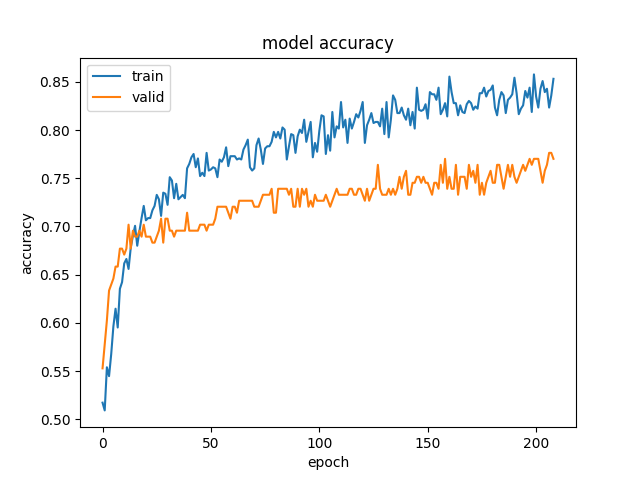
\includegraphics[width =2.5in]{images/appendice/stl/incnet/accuracy.png}} 
\subfloat[Loss]{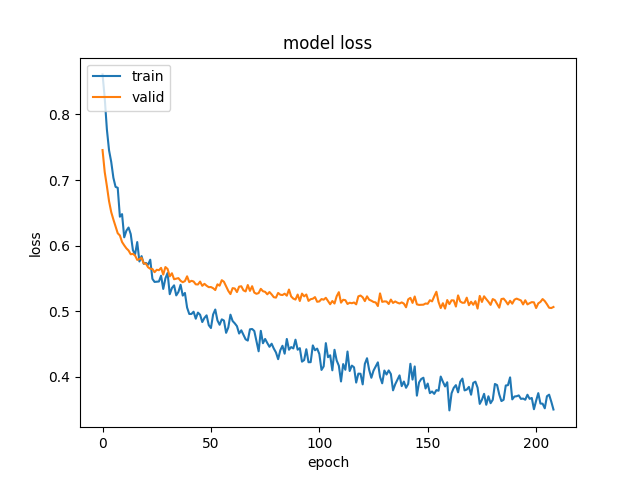
\includegraphics[width = 2.5in]{images/appendice/stl/incnet/loss.png}}\\
\caption{Training Curves for Single-Task learning model with $IncNet$. The y-axis indicates the metric fuction. The x-axis indicates the epochs of training.}
\label{incNettraining}
\end{figure}
\begin{figure}[ht]
\centering
{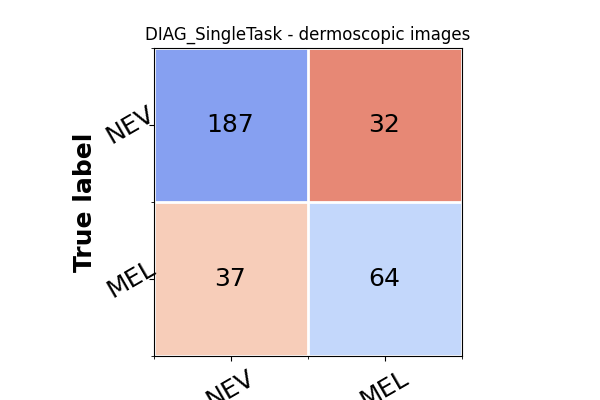
\includegraphics[width =2.5in]{images/appendice/stl/incnet/DIAG_CM_SingleTask.png}}
\caption{Confusion matrix for DIAG task using the test set prediction
from the $IncNet$ model. The y-axis indicates the ground truth labels. The x-axis indicates the model’s predicted labels. Numbers in each entry represent
the number of cases classified as such. Colors indicate the percentage of each
label in each entry, normalized by the total number of true labels.}
\label{incNetCM}
\end{figure}
\clearpage
\subsection{\texorpdfstring{\boldsymbol{$ResNet$}}{TEXT}}
\label{ResNet}
\begin{figure}[ht]
\subfloat[Accuracy]{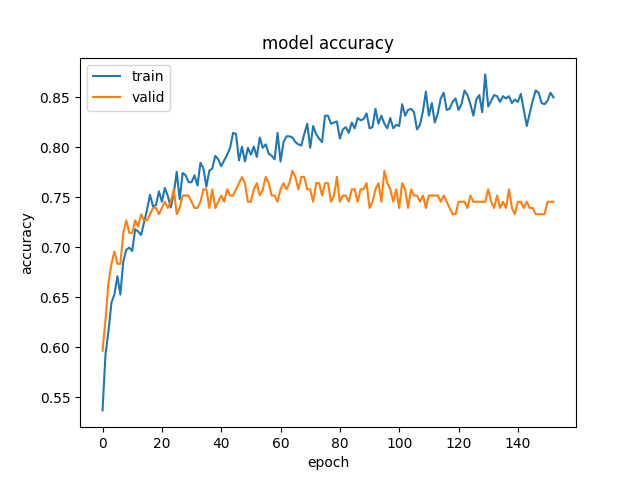
\includegraphics[width =2.5in]{images/appendice/stl/resnet/accuracy.png}} 
\subfloat[Loss]{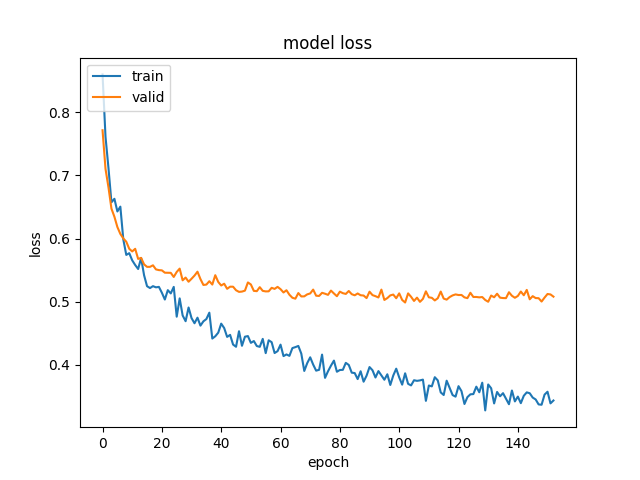
\includegraphics[width = 2.5in]{images/appendice/stl/resnet/loss.png}}\\
\caption{Training Curves for Single-Task learning model with $ResNet$. The y-axis indicates the metric fuction. The x-axis indicates the epochs of training}
\label{resNettraining}
\end{figure}
\begin{figure}[ht]
\centering
{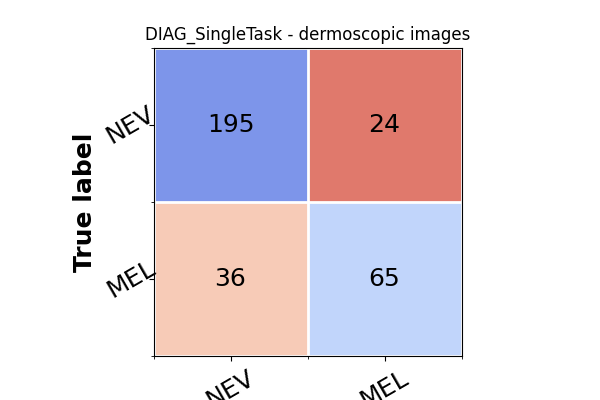
\includegraphics[width =2.5in]{images/appendice/stl/resnet/DIAG_CM_SingleTask.png}}
\caption{Confusion matrix for DIAG task using the test set prediction
from the $ResNet$ model. The y-axis indicates the ground truth labels. The x-axis indicates the model’s predicted labels. Numbers in each entry represent
the number of cases classified as such. Colors indicate the percentage of each
label in each entry, normalized by the total number of true labels.}
\label{resNetCM}
\end{figure}
\clearpage
\subsection{\texorpdfstring{\boldsymbol{$IncNet^*+L.R.$}}{TEXT}}
\begin{figure}[ht]
\centering
{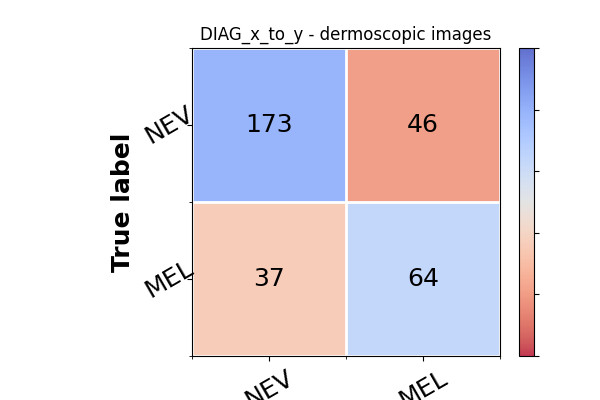
\includegraphics[width =2.5in]{images/appendice/stl/incnet+lr/DIAG_CM_x_to_y.png}}
\caption{Confusion matrix for DIAG task using the test set prediction
from the $IncNet^*+L.R.$ model. The y-axis indicates the ground truth labels. The x-axis indicates the model’s predicted labels. Numbers in each entry represent
the number of cases classified as such. Colors indicate the percentage of each
label in each entry, normalized by the total number of true labels.}
\label{incNet+lrCM}
\end{figure}

\subsection{\texorpdfstring{\boldsymbol{$ResNet^*+L.R.$}}{TEXT}}
\begin{figure}[ht]
\centering
{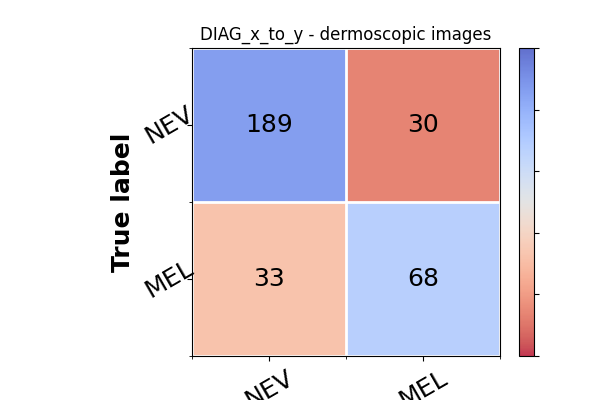
\includegraphics[width =2.5in]{images/appendice/stl/resnet+lr/DIAG_CM_x_to_y.png}}
\caption{Confusion matrix for DIAG task using the test set prediction
from the $ResNet^*+L.R.$ model. The y-axis indicates the ground truth labels. The x-axis indicates the model’s predicted labels. Numbers in each entry represent
the number of cases classified as such. Colors indicate the percentage of each
label in each entry, normalized by the total number of true labels.}
\label{resNet+lrCM}
\end{figure}



\clearpage

\section{Multi-Task Learning}

\subsection{\texorpdfstring{\boldsymbol{$IncNet_{MTL}$}}{TEXT}}
\label{MtlIncNet}
\begin{figure}[ht]
\subfloat[Accuracy]{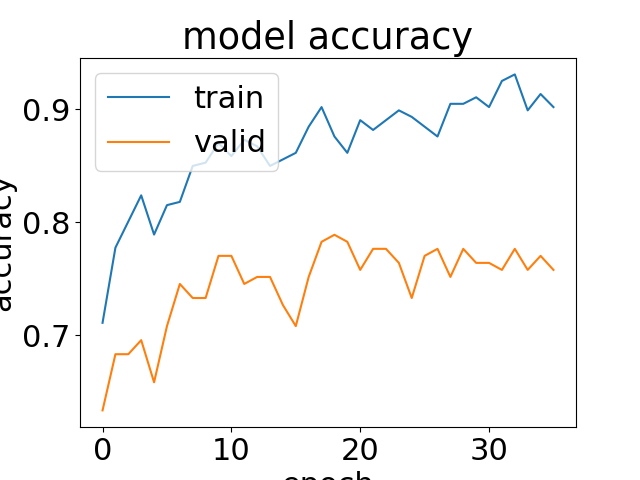
\includegraphics[width =2.5in]{images/appendice/mtl/accuracy/accuracy.png}} 
\subfloat[Loss]{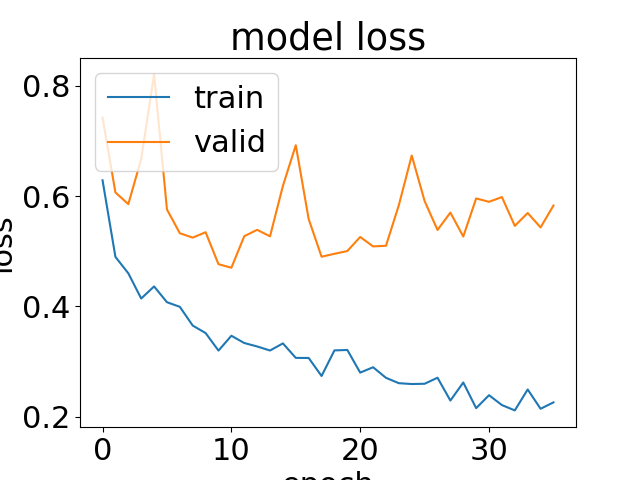
\includegraphics[width = 2.5in]{images/appendice/mtl/loss/loss.png}}

\caption{Training Curves for Multi-Task learning model with $IncNet$. The y-axis indicates the metric fuction. The x-axis indicates the epochs of training}
\label{MTLtraining}
\end{figure}

\begin{figure}[ht]
\centering
\subfloat[BWV]{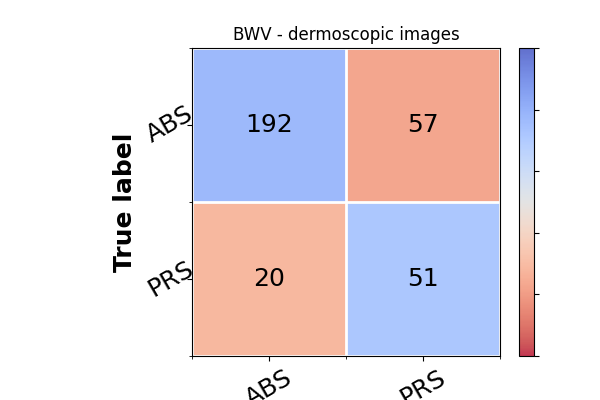
\includegraphics[width =2in]{images/appendice/mtl/CM/BWV_CM.png}} 
\subfloat[DaG]{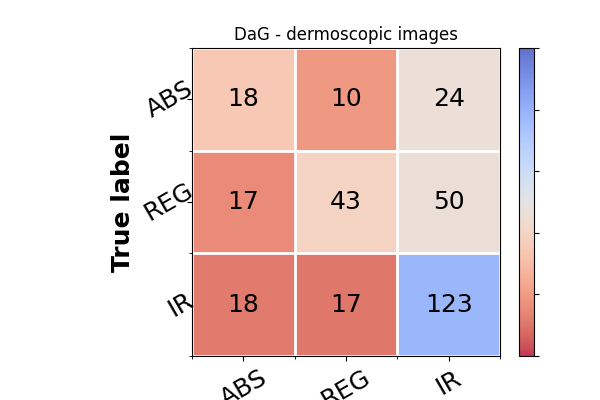
\includegraphics[width = 2in]{images/appendice/mtl/CM/DaG_CM.png}}
\subfloat[PIG]{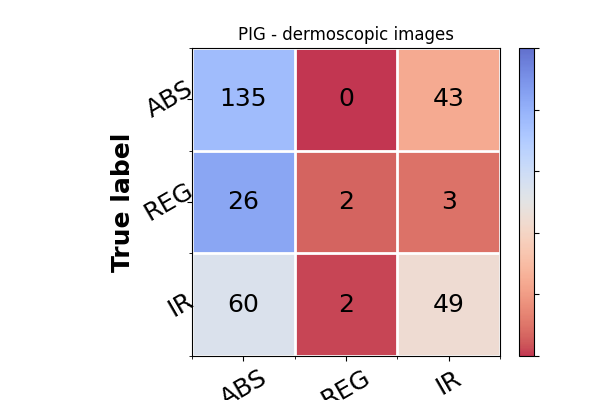
\includegraphics[width = 2in]{images/appendice/mtl/CM/PIG_CM.png}}\\
\subfloat[PN]{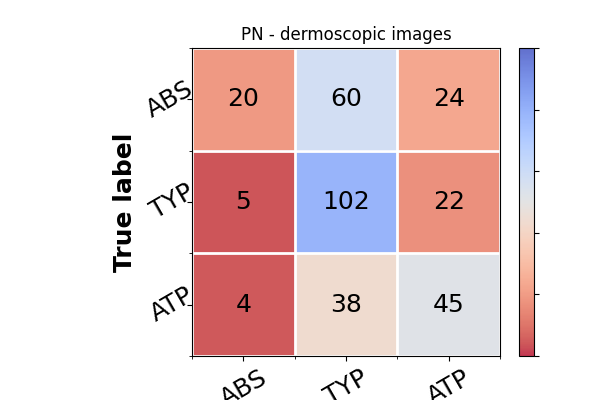
\includegraphics[width = 2in]{images/appendice/mtl/CM/PN_CM.png}} 
\subfloat[VS]{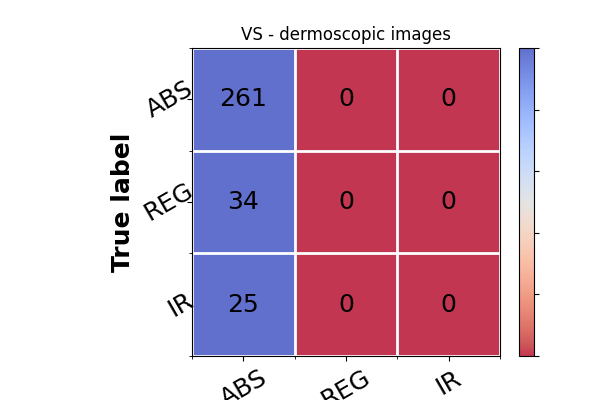
\includegraphics[width = 2in]{images/appendice/mtl/CM/VS_CM.png}}
\subfloat[STR]{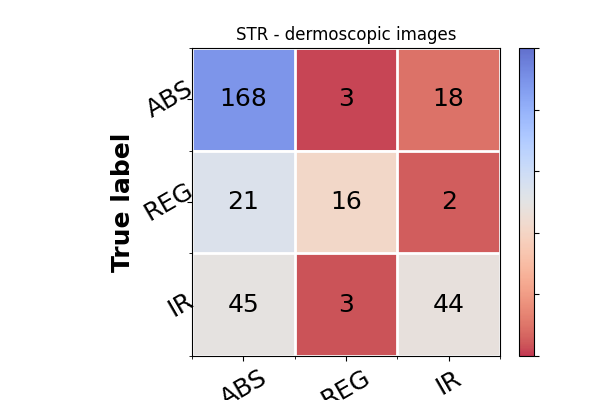
\includegraphics[width = 2in]{images/appendice/mtl/CM/STR_CM.png}}\\
\subfloat[RS]{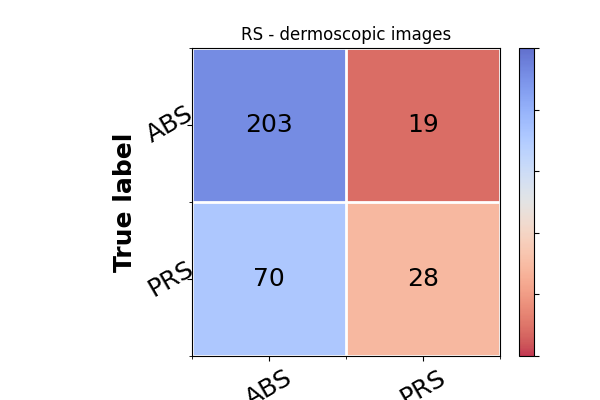
\includegraphics[width = 2in]{images/appendice/mtl/CM/RS_CM.png}} 
\caption{Confusion matrices for each concepts using the test set predictions
from the $IncNet_{MTL}$ model. The y-axis indicates the ground truth labels. The
x-axis indicates the model’s predicted labels. Numbers in each entry represent
the number of cases classified as such. Colors indicate the percentage of each
label in each entry, normalized by the total number of true labels.}
\label{CMincNetMTL}
\end{figure}

\clearpage

\subsection{\texorpdfstring{\boldsymbol{$IncNet^*_{MTL}+L.R.$}}{TEXT}}
\begin{figure}[ht]
\centering
\subfloat[BWV]{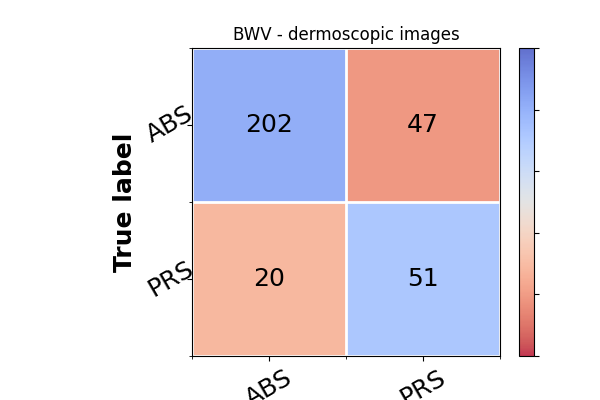
\includegraphics[width =2in]{images/appendice/incnet+lr/CM/BWV_CM.png}} 
\subfloat[DaG]{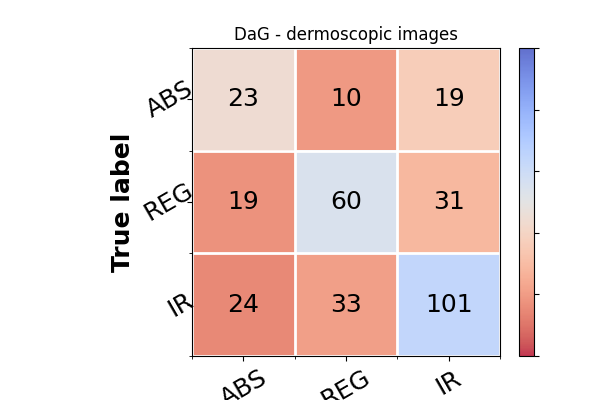
\includegraphics[width = 2in]{images/appendice/incnet+lr/CM/DaG_CM.png}}
\subfloat[PIG]{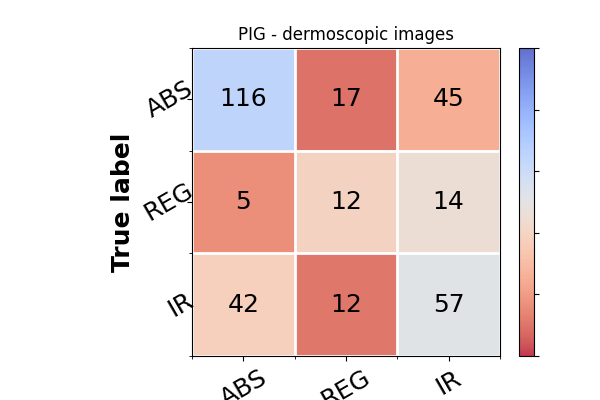
\includegraphics[width = 2in]{images/appendice/incnet+lr/CM/PIG_CM.png}}\\
\subfloat[PN]{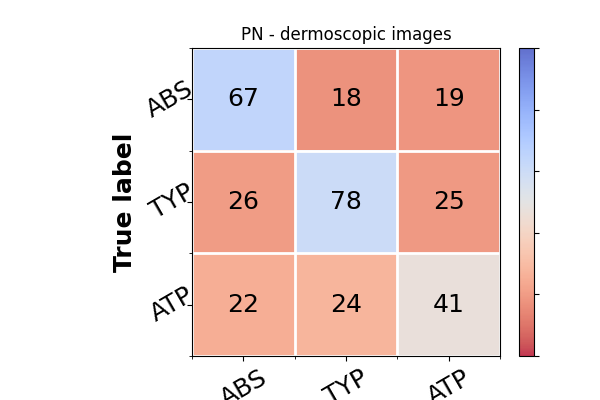
\includegraphics[width = 2in]{images/appendice/incnet+lr/CM/PN_CM.png}} 
\subfloat[VS]{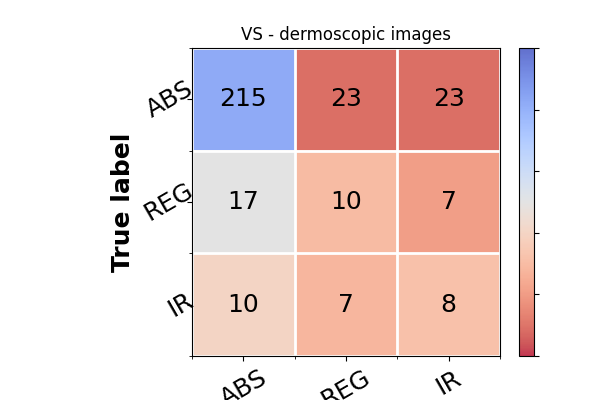
\includegraphics[width = 2in]{images/appendice/incnet+lr/CM/VS_CM.png}}
\subfloat[STR]{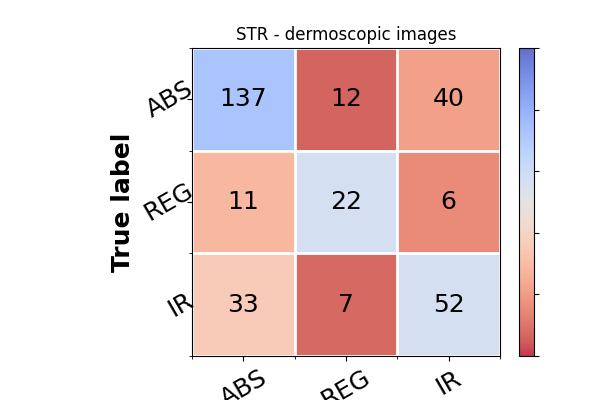
\includegraphics[width = 2in]{images/appendice/incnet+lr/CM/STR_CM.png}}\\
\subfloat[RS]{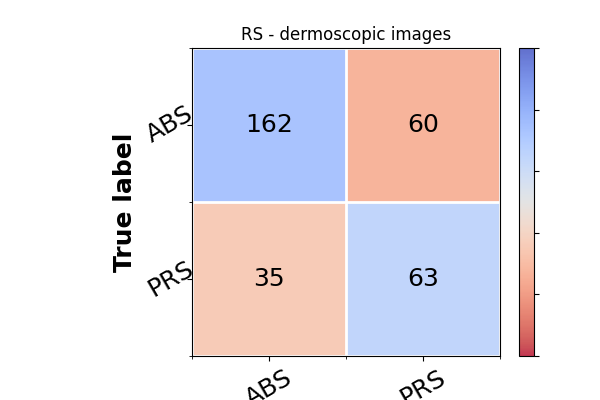
\includegraphics[width = 2in]{images/appendice/incnet+lr/CM/RS_CM.png}} 
\caption{Confusion matrices for each concepts using the test set predictions
from the $IncNet^*_{MTL}+L.R.$ model. The y-axis indicates the ground truth labels. The x-axis indicates the model’s predicted labels. Numbers in each entry represent
the number of cases classified as such. Colors indicate the percentage of each
label in each entry, normalized by the total number of true labels.}
\label{CMincNetMTLLR}
\end{figure}
\clearpage
\subsection{\texorpdfstring{\boldsymbol{$ResNet^*_{MTL}+L.R.$}}{TEXT}} 
\begin{figure}[ht]
\centering
\subfloat[BWV]{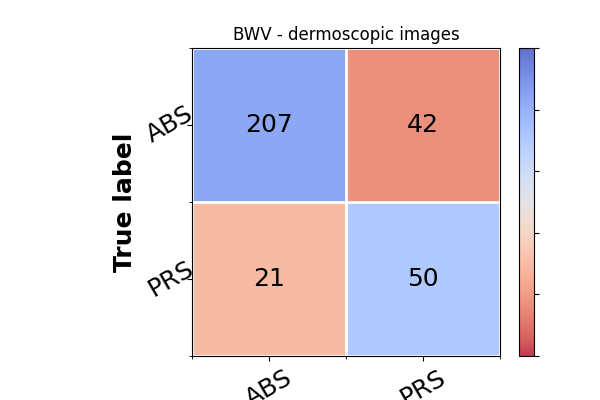
\includegraphics[width =2in]{images/appendice/resnet+lr/CM/BWV_CM.png}} 
\subfloat[DaG]{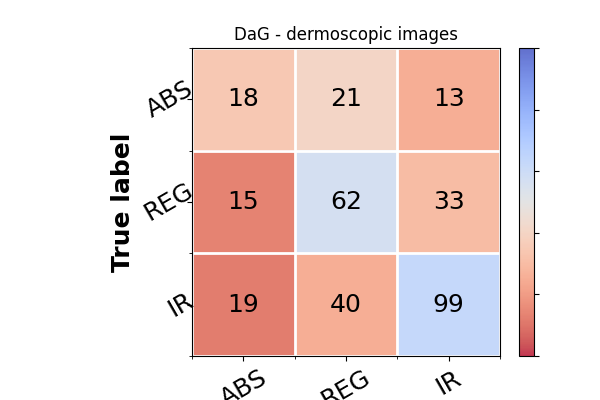
\includegraphics[width = 2in]{images/appendice/resnet+lr/CM/DaG_CM.png}}
\subfloat[PIG]{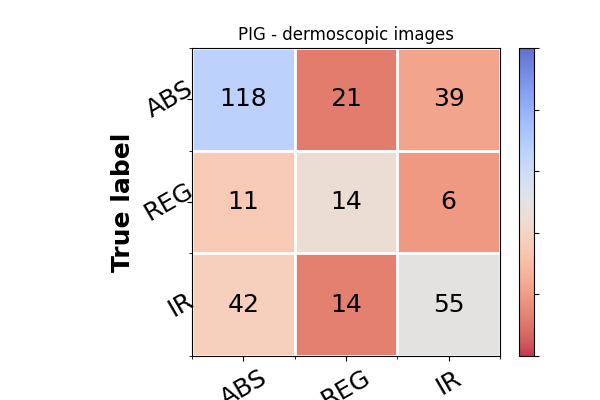
\includegraphics[width = 2in]{images/appendice/resnet+lr/CM/PIG_CM.png}}\\
\subfloat[PN]{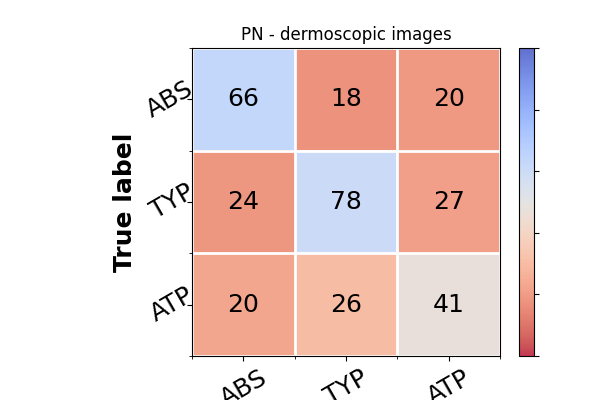
\includegraphics[width = 2in]{images/appendice/resnet+lr/CM/PN_CM.png}}
\subfloat[VS]{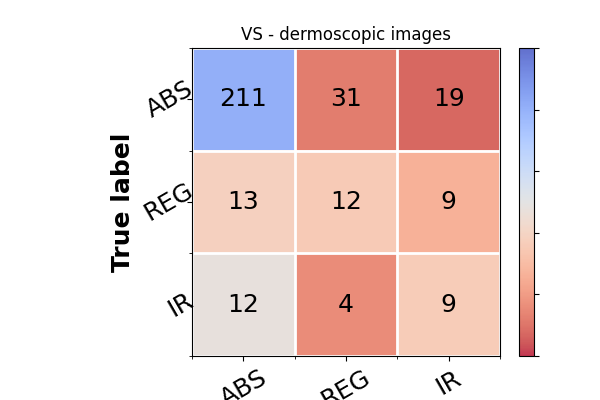
\includegraphics[width = 2in]{images/appendice/resnet+lr/CM/VS_CM.png}}
\subfloat[STR]{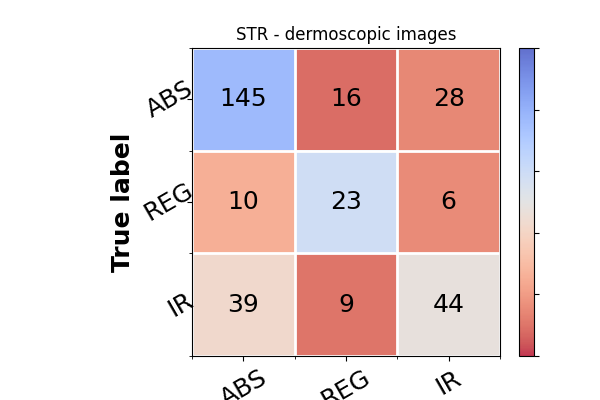
\includegraphics[width = 2in]{images/appendice/resnet+lr/CM/STR_CM.png}}\\
\subfloat[RS]{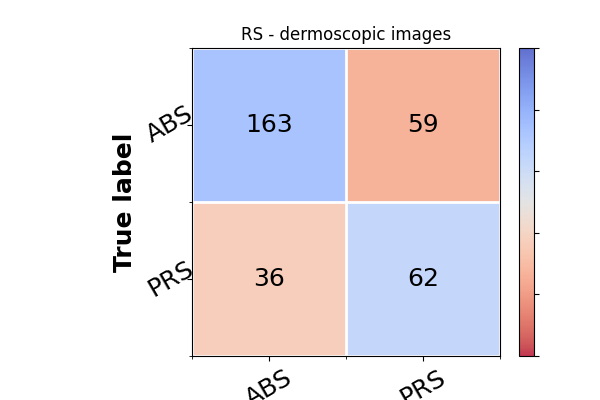
\includegraphics[width = 2in]{images/appendice/resnet+lr/CM/RS_CM.png}} 
\caption{Confusion matrices for each concepts using the test set predictions
from the $ResNet^*_{MTL}+L.R.$ model. The y-axis indicates the ground truth labels. The x-axis indicates the model’s predicted labels. Numbers in each entry represent
the number of cases classified as such. Colors indicate the percentage of each
label in each entry, normalized by the total number of true labels.}
\label{CMincNetMTLLR}
\end{figure}

\clearpage
\section{Concept-Bottleneck Models}

\subsection{\texorpdfstring{\boldsymbol{$Ind|IncNet_{MTL}$}}{TEXT}}
\begin{figure}[ht]
\centering
{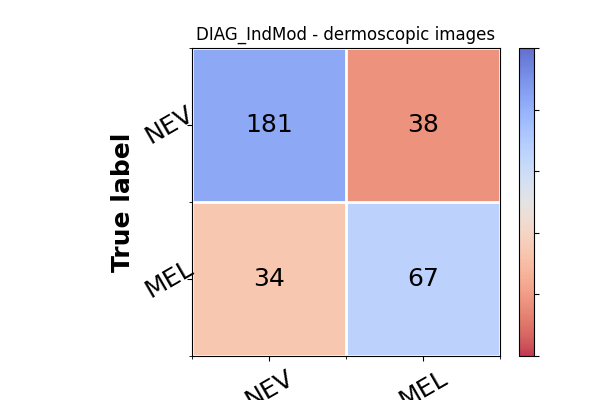
\includegraphics[width =2.5in]{images/appendice/mtl/DIAG_CM_IndMod.png}}
\caption{Confusion matrix for DIAG task using the test set prediction
from the $Ind|IncNet_{MTL}$ model. The y-axis indicates the ground truth labels. The x-axis indicates the model’s predicted labels. Numbers in each entry represent
the number of cases classified as such. Colors indicate the percentage of each
label in each entry, normalized by the total number of true labels.}
\label{IndincNetCM}
\end{figure}

\subsection{\texorpdfstring{\boldsymbol{$Seq|IncNet_{MTL}$}}{TEXT}}
\begin{figure}[ht]
\centering
{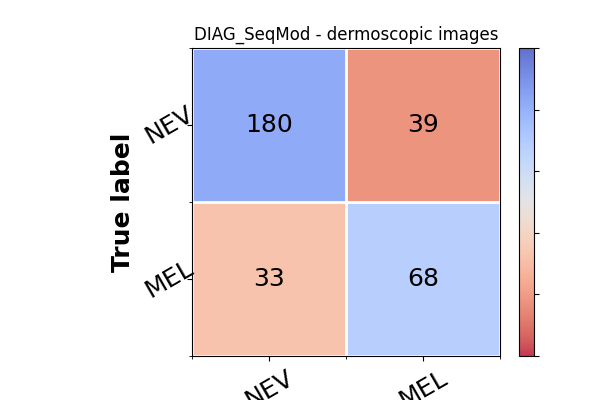
\includegraphics[width =2.5in]{images/appendice/mtl/DIAG_CM_SeqMod.png}}
\caption{Confusion matrix for DIAG task using the test set prediction
from the $Seq|IncNet_{MTL}$ model. The y-axis indicates the ground truth labels. The x-axis indicates the model’s predicted labels. Numbers in each entry represent
the number of cases classified as such. Colors indicate the percentage of each
label in each entry, normalized by the total number of true labels.}
\label{SeqincNetCM}
\end{figure}
\clearpage

\subsection{\texorpdfstring{\boldsymbol{$Ind|IncNet^*_{MTL}+L.R.$}}{TEXT}}
\begin{figure}[ht]
\centering
{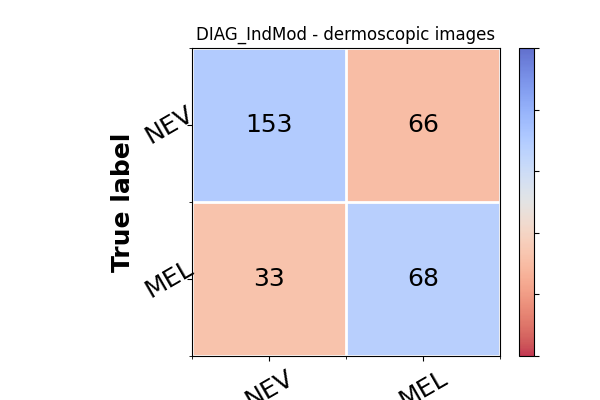
\includegraphics[width =2.5in]{images/appendice/incnet+lr/DIAG_CM_IndMod.png}}
\caption{Confusion matrix for DIAG task using the test set prediction
from the $Ind|IncNet^*_{MTL}+L.R.$ model. The y-axis indicates the ground truth labels. The x-axis indicates the model’s predicted labels. Numbers in each entry represent
the number of cases classified as such. Colors indicate the percentage of each
label in each entry, normalized by the total number of true labels. }
\label{IndincNet+lrCM}
\end{figure}

\subsection{\texorpdfstring{\boldsymbol{$Ind|ResNet^*_{MTL}+L.R.$}}{TEXT}}
\begin{figure}[ht]
\centering
{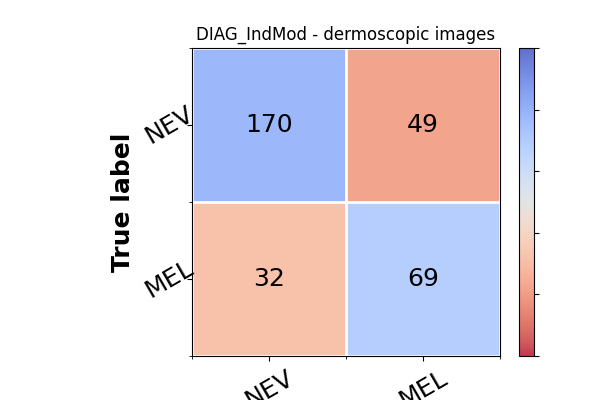
\includegraphics[width =2.5in]{images/appendice/resnet+lr/DIAG_CM_IndMod.png}}
\caption{Confusion matrix for DIAG task using the test set prediction
from the $Ind|ResNet^*_{MTL}+L.R.$ model. The y-axis indicates the ground truth labels. The x-axis indicates the model’s predicted labels. Numbers in each entry represent
the number of cases classified as such. Colors indicate the percentage of each
label in each entry, normalized by the total number of true labels.}
\label{IndresNet+lrCM}
\end{figure}
\clearpage

\subsection{\texorpdfstring{\boldsymbol{$Seq|IncNet^*_{MTL}+L.R.$}}{TEXT}}
\begin{figure}[ht]
\centering
{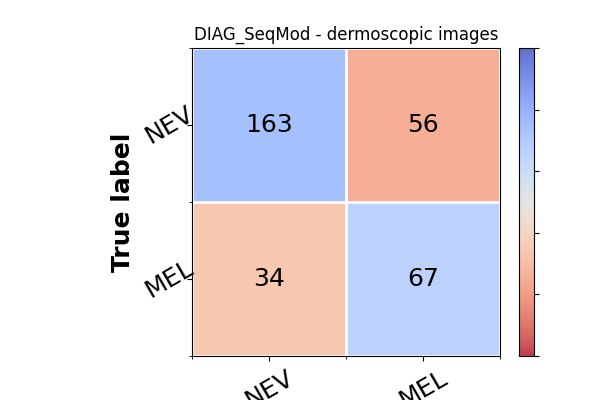
\includegraphics[width =2.5in]{images/appendice/incnet+lr/DIAG_CM_SeqMod.png}}
\caption{Confusion matrix for DIAG task using the test set prediction
from the $Seq|IncNet^*_{MTL}+L.R.$ model. The y-axis indicates the ground truth labels. The x-axis indicates the model’s predicted labels. Numbers in each entry represent
the number of cases classified as such. Colors indicate the percentage of each
label in each entry, normalized by the total number of true labels.}
\label{SeqincNet+lrCM}
\end{figure}

\subsection{\texorpdfstring{\boldsymbol{$Seq|ResNet^*_{MTL}+L.R.$}}{TEXT}}
\begin{figure}[ht]
\centering
{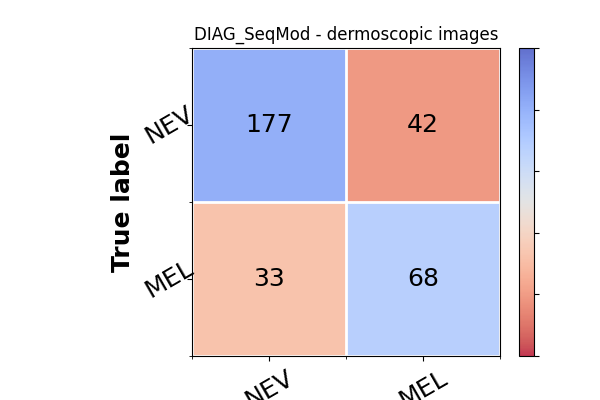
\includegraphics[width =2.5in]{images/appendice/resnet+lr/DIAG_CM_SeqMod.png}}
\caption{Confusion matrix for DIAG task using the test set prediction
from the $Seq|ResNet^*_{MTL}+L.R.$ model. The y-axis indicates the ground truth labels. The x-axis indicates the model’s predicted labels. Numbers in each entry represent
the number of cases classified as such. Colors indicate the percentage of each
label in each entry, normalized by the total number of true labels.}
\label{SeqresNet+lrCM}
\end{figure}
\clearpage
\section{7-pt Checklist Rule}
\begin{figure}[ht]
\centering
{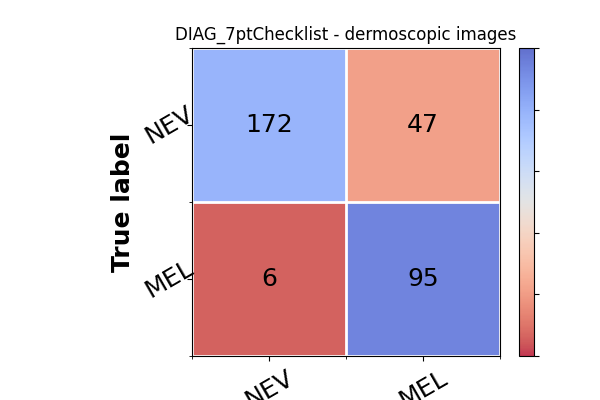
\includegraphics[width =2.5in]{images/appendice/DIAG_CM_7pt_trueC.png}}
\caption{Confusion matrix for DIAG task using the test set prediction
from the 7-pt Checlist Rule. The y-axis indicates the ground truth labels. The x-axis indicates the model’s predicted labels. Numbers in each entry represent
the number of cases classified as such. Colors indicate the percentage of each
label in each entry, normalized by the total number of true labels.}
\label{7ptCm}
\end{figure}